%%%%%%%%%%%%%%%%%%%%%%%%%%%%%%%%%%%%%%%%%%%%%%%%%%%%%%
% A template for Wiley article submissions.
% Developed by Overleaf. 
%
% Please note that whilst this template provides a 
% preview of the typeset manuscript for submission, it 
% will not necessarily be the final publication layout.
%
% Usage notes:
% The "blind" option will make anonymous all author, affiliation, correspondence and funding information.
% Use "num-refs" option for numerical citation and references style.
% Use "alpha-refs" option for author-year citation and references style.

\documentclass[num-refs]{wiley-article}
% \documentclass[blind,alpha-refs]{wiley-article}

% added for highlighting
\usepackage{soul}

% added for margin notes
\usepackage{marginnote}

\bibliographystyle{vancouver-authoryear}

% Add additional packages here if required
\usepackage{siunitx}

% Graphics. Always show the figures but float to the end
% code listing
\usepackage[final]{subfig, listings}
\usepackage[nofiglist]{endfloat}

\graphicspath{{./figures/}}

% Update article type if known
\papertype{Full paper}
% Include section in journal if known, otherwise delete
% \paperfield{Journal Section}

\title{Adaptive Baseline Fitting for $^{\textbf{1}}$H MR Spectroscopy Analysis}

% Use the \authfn to add symbols for additional footnotes and present addresses, if any. Usually start with 1 for notes about author contributions; then continuing with 2 etc if any author has a different present address.
\author[1]{Martin Wilson}

%\contrib[\authfn{1}]{Equally contributing authors.}

% Include full affiliation details for all authors
\affil[1]{Centre for Human Brain Health and School of Psychology, University of Birmingham, Birmingham, UK.}

\corraddress{Martin Wilson, Centre for Human Brain Health, University of Birmingham, Edgbaston, Birmingham, B15 2TT, United Kingdom.}

\corremail{wilsonmp@bham.ac.uk}

% \fundinginfo{Funder One, Funder One Department, Grant/Award Number: 123456, 123457 and 123458; Funder Two, Funder Two Department, Grant/Award Number: 123459}

% Include the name of the author that should appear in the running header
\runningauthor{Wilson}

% my macros
\newcommand{\proton}{\ensuremath{^1\mathrm{H}}}
\newcommand{\bzero}{\ensuremath{\mathrm{B}_0}}
\soulregister\bzero7 % needed for soul to work with this macro
\soulregister\ref7 % needed for soul to work with this macro
\soulregister\cite7 % needed for soul to work with this macro

% revision two highlighting
%\newcommand{\revtwo}[2]{\hl{#1}\marginnote{\hl{#2}}}
%\newcommand{\revtwonm}[1]{\hl{#1}} % no margin label

% uncomment next two lines to hide revision two highlighting
%\newcommand{\revtwo}[2]{#1}
%\newcommand{\revtwonm}[1]{#1}

\begin{document}

\maketitle

\begin{abstract}
\textbf{Purpose:} \\
\textbf{Methods:} \\
\textbf{Results:} \\
\textbf{Conclusion:} 
\keywords{XXXX}
\end{abstract}

Word count : XXXX

% MRM abstract max length is 250 words
% MRM note max length is 2800 words, 5 fig plus tables

\section{Introduction}
A number of key metabolites may be detected using \proton\ Magnetic Resonance Spectroscopy (MRS), providing a non-invasive measure of healthy and diseased brain tissue metabolism. Clinical applications include the assessment of brain tumors, metabolic disorders and neonatal encephalopathy \cite{Oz2014,Lally2019} where the concentration of certain metabolites may inform disease diagnosis or predict patient outcome. Further applications for MRS are present in the neuroscience and psychiatry domains, with particular interest in the direct detection of neurotransmitter levels such as GABA and glutamate, which have been shown to be abnormal in Schizophrenia \cite{Merritt2016} and modulate in response to tasks \cite{Jelen2018,Chen2017}.

MRS scans are typically performed at short (30ms) or long (144ms) TE's, with short-TE scans being preferred due to reduced T2 relaxation and dephasing of multiplets resulting in improved metabolite detection sensitivity \cite{Wilson2019}. However, short-TE scans are typically more susceptible to artifacts originating from insufficient water and scalp lipid suppression, in addition, broad signals from macromolecules also become enhanced \cite{Cudalbu2012}. Residual water signals, lipid signals and macromolecules all have the potential to bias metabolite measurements due to spectral overlap and interference. Therefore, appropriate analysis methodology is particularly important to achieve the full benefit of conventional short-TE MRS.

Parametric fitting is currently the most widely used analysis method for MRS data, and typically incorporates a set of simulated metabolite signals - known as a basis set. One of the main distinctions between analysis methods is their approach for mitigating metabolite estimation bias from broad signals not present in the basis set, usually referred to as "baseline modeling". One of the most popular baseline modeling methods incorporates a set of smooth spline functions into the fitting procedure, with additional smoothness imposed by penalizing greater baseline complexity. The LCModel \cite{Provencher1993} and AQSES \cite{Poullet2007} algorithms both use penalized spline baseline modeling, with analysis performed in the frequency-domain and time-domain respectively. 

An alternative approach to baseline modeling exploits the rapid decay of baseline signals in the time-domain by omitting the preliminary data points during the fitting process, reducing their interference with the more slowly decaying metabolites. The QUEST \cite{Ratiney2005} and TARQUIN \cite{Wilson2011} methods both use this time-domain truncation approach. The FITT \cite{Young1998} algorithm combines the wavelet transform with Lowess filtering in the frequency-domain to separate metabolite and baseline signals.

Control over the level of baseline flexibility (or smoothness) is a common and necessary requirement of each of the baseline modeling methods outlined above. For spline based approaches, the number of spline functions for a given frequency range and the smoothness penalty parameter control the baseline flexibility. For LCModel, the frequency spacing between the spline basis functions is dependent on data quality, and is set at maximum of 1.5 times the estimated full width at half maximum (FWHM) of the metabolite resonances or 0.1 ppm \cite{Provencher1993}. Similarly, for the FITT algorithm a fixed Lowess filter smoothing value is used and wavelet coefficients with scales less than twice the FWHM are excluded from the baseline model to ensure smoothness \cite{Young1998}. In the time-domain truncation approach baseline flexibility is primarily determined by the number of initial data points to be omitted from the fit evaluation. For QUEST and TARQUIN the number of truncated data points, and therefore degree of baseline flexibility, is set at a default value that may be adjusted by the user. 

Automated methods to determine the correct degree of baseline flexibility are important for obtaining accurate metabolite levels independently of the analyst. Furthermore, the manual adjustment of baseline flexibility for each individual spectrum is impractical for MRSI studies - where hundreds of spectra may be acquired in a single scan. Whilst LCModel provides automated adjustment of baseline flexibility, a growing number of analysts choose to manually override the default analysis settings by adjusting the spline spacing parameter (DKNTMN). The first reported use of this manual adjustment was to improve the modeling of macromolecular resonances in rat brain at 9.4 T \cite{Pfeuffer1999}. More recently, this parameter has been adjusted to encourage flatter baselines \cite{Deelchand2016,Terpstra2010,Marjanska2018}, suggesting the default LCModel baseline flexibility may not be optimal in some cases. 

Finding the optimal degree of baseline flexibility is a crucial question in MRS analysis research, yet few studies have investigated this topic in detail. Using simulated data, Ratiney et al. demonstrated how the interference between metabolite and baseline signals was reduced by increasing the number of omitted data points, but this came at the cost of inflating errors due to noise \cite{Ratiney2004}. More recently, Near et al. showed how the estimated baseline in LCModel can depend strongly on spectral SNR and metabolite FWHM, and that errors caused by baseline instability may dominate over errors from spectral noise in some cases \cite{Near2013}. The influence of baseline flexibility has also been explored using experimentally acquired data, with a recent study demonstrating a 15\% difference in metabolite levels when comparing between a default and less flexible baseline model \cite{Giapitzakis2019}. Baseline flexibility has also been shown to have a strong influence of the measurement of 2-hydroxyglutarate \cite{Wenger2019}.

In this study we introduce a new method to automatically determine the optimal degree of baseline flexibility for a frequency-domain spline based fitting algorithm. Firstly, background is given on the use of penalized splines for optimal data smoothing. A fully-automated fitting algorithm is presented, incorporating a novel method to automatically estimate the optimal level of baseline flexibility. Finally, the new method is validated on simulated and experimentally acquired MRSI data.

\section{Methods}
\subsection{Penalized spline regression}

Baseline signals have a characteristically smooth spectral appearance, and must to be accurately modeled to avoid biasing metabolite estimates. In good quality \proton\ MRS of brain tissue baseline signals have a low intensity, relative to the primary metabolite resonances, and are therefore challenging to estimate in the presence of noise. Estimating a smooth function from noisy data is known in statistics as ``scatterplot smoothing'', and a number of approaches have been developed \cite{Ruppert2003}. In this section we briefly outline the method of penalized splines in the simpler context of scatterplot smoothing, before describing their use as part of an MRS fitting algorithm.

% Figure 1
\begin{figure}
  \begin{center}
    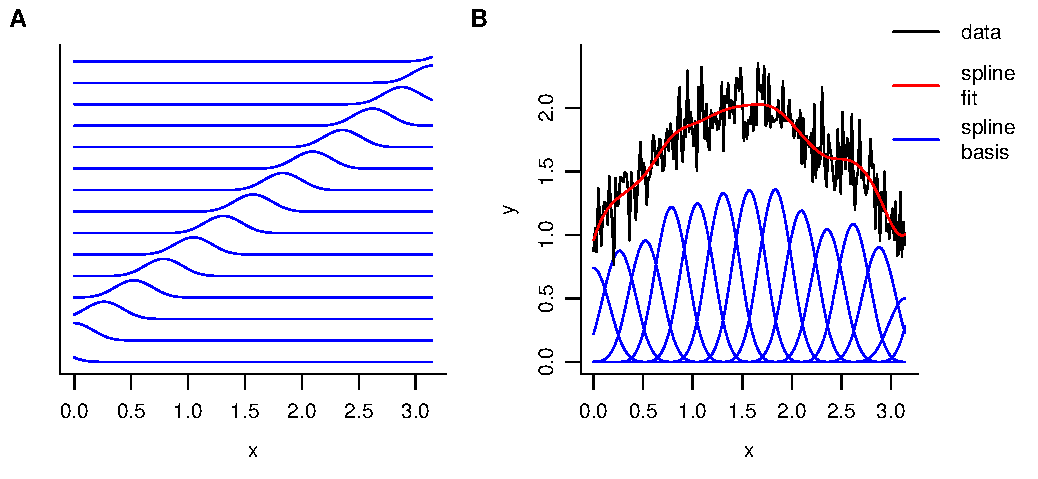
\includegraphics[width=0.9\textwidth]{fig1.pdf}
    \caption{xxx}
    \label{yyy}
  \end{center}
\end{figure}

XXXX

\section{Results}
XXXX

\section{Discussion}
MRM open science paper: https://onlinelibrary.wiley.com/doi/full/10.1002/mrm.27939

XXXX

\section{Conclusion}
XXXX

\section*{ACKNOWLEDGEMENTS}
XXXX

\bibliography{main}

\clearpage
\listoffigures

\end{document}

%%% Local Variables:
%%% mode: latex
%%% eval: (spacemacs/toggle-visual-line-navigation-on)
%%% eval: (spacemacs/toggle-auto-fill-mode-off)
%%% End: